% Options for packages loaded elsewhere
\PassOptionsToPackage{unicode}{hyperref}
\PassOptionsToPackage{hyphens}{url}
%
\documentclass[
  english,
  ,man,floatsintext]{apa6}
\usepackage{lmodern}
\usepackage{amsmath}
\usepackage{ifxetex,ifluatex}
\ifnum 0\ifxetex 1\fi\ifluatex 1\fi=0 % if pdftex
  \usepackage[T1]{fontenc}
  \usepackage[utf8]{inputenc}
  \usepackage{textcomp} % provide euro and other symbols
  \usepackage{amssymb}
\else % if luatex or xetex
  \usepackage{unicode-math}
  \defaultfontfeatures{Scale=MatchLowercase}
  \defaultfontfeatures[\rmfamily]{Ligatures=TeX,Scale=1}
\fi
% Use upquote if available, for straight quotes in verbatim environments
\IfFileExists{upquote.sty}{\usepackage{upquote}}{}
\IfFileExists{microtype.sty}{% use microtype if available
  \usepackage[]{microtype}
  \UseMicrotypeSet[protrusion]{basicmath} % disable protrusion for tt fonts
}{}
\makeatletter
\@ifundefined{KOMAClassName}{% if non-KOMA class
  \IfFileExists{parskip.sty}{%
    \usepackage{parskip}
  }{% else
    \setlength{\parindent}{0pt}
    \setlength{\parskip}{6pt plus 2pt minus 1pt}}
}{% if KOMA class
  \KOMAoptions{parskip=half}}
\makeatother
\usepackage{xcolor}
\IfFileExists{xurl.sty}{\usepackage{xurl}}{} % add URL line breaks if available
\IfFileExists{bookmark.sty}{\usepackage{bookmark}}{\usepackage{hyperref}}
\hypersetup{
  pdftitle={What might books be teaching young children about gender?},
  pdfauthor={Molly Lewis1,2, Matt Cooper Borkenhagen3, Erin Converse3, Gary Lupyan3, \& Mark S. Seidenberg3},
  pdflang={en-EN},
  pdfkeywords={reading, gender, language development},
  hidelinks,
  pdfcreator={LaTeX via pandoc}}
\urlstyle{same} % disable monospaced font for URLs
\usepackage{graphicx}
\makeatletter
\def\maxwidth{\ifdim\Gin@nat@width>\linewidth\linewidth\else\Gin@nat@width\fi}
\def\maxheight{\ifdim\Gin@nat@height>\textheight\textheight\else\Gin@nat@height\fi}
\makeatother
% Scale images if necessary, so that they will not overflow the page
% margins by default, and it is still possible to overwrite the defaults
% using explicit options in \includegraphics[width, height, ...]{}
\setkeys{Gin}{width=\maxwidth,height=\maxheight,keepaspectratio}
% Set default figure placement to htbp
\makeatletter
\def\fps@figure{htbp}
\makeatother
\setlength{\emergencystretch}{3em} % prevent overfull lines
\providecommand{\tightlist}{%
  \setlength{\itemsep}{0pt}\setlength{\parskip}{0pt}}
\setcounter{secnumdepth}{-\maxdimen} % remove section numbering
% Make \paragraph and \subparagraph free-standing
\ifx\paragraph\undefined\else
  \let\oldparagraph\paragraph
  \renewcommand{\paragraph}[1]{\oldparagraph{#1}\mbox{}}
\fi
\ifx\subparagraph\undefined\else
  \let\oldsubparagraph\subparagraph
  \renewcommand{\subparagraph}[1]{\oldsubparagraph{#1}\mbox{}}
\fi
% Manuscript styling
\usepackage{upgreek}
\captionsetup{font=singlespacing,justification=justified}

% Table formatting
\usepackage{longtable}
\usepackage{lscape}
% \usepackage[counterclockwise]{rotating}   % Landscape page setup for large tables
\usepackage{multirow}		% Table styling
\usepackage{tabularx}		% Control Column width
\usepackage[flushleft]{threeparttable}	% Allows for three part tables with a specified notes section
\usepackage{threeparttablex}            % Lets threeparttable work with longtable

% Create new environments so endfloat can handle them
% \newenvironment{ltable}
%   {\begin{landscape}\begin{center}\begin{threeparttable}}
%   {\end{threeparttable}\end{center}\end{landscape}}
\newenvironment{lltable}{\begin{landscape}\begin{center}\begin{ThreePartTable}}{\end{ThreePartTable}\end{center}\end{landscape}}

% Enables adjusting longtable caption width to table width
% Solution found at http://golatex.de/longtable-mit-caption-so-breit-wie-die-tabelle-t15767.html
\makeatletter
\newcommand\LastLTentrywidth{1em}
\newlength\longtablewidth
\setlength{\longtablewidth}{1in}
\newcommand{\getlongtablewidth}{\begingroup \ifcsname LT@\roman{LT@tables}\endcsname \global\longtablewidth=0pt \renewcommand{\LT@entry}[2]{\global\advance\longtablewidth by ##2\relax\gdef\LastLTentrywidth{##2}}\@nameuse{LT@\roman{LT@tables}} \fi \endgroup}

% \setlength{\parindent}{0.5in}
% \setlength{\parskip}{0pt plus 0pt minus 0pt}

% \usepackage{etoolbox}
\makeatletter
\patchcmd{\HyOrg@maketitle}
  {\section{\normalfont\normalsize\abstractname}}
  {\section*{\normalfont\normalsize\abstractname}}
  {}{\typeout{Failed to patch abstract.}}
\patchcmd{\HyOrg@maketitle}
  {\section{\protect\normalfont{\@title}}}
  {\section*{\protect\normalfont{\@title}}}
  {}{\typeout{Failed to patch title.}}
\makeatother
\shorttitle{Gender in children's books}
\keywords{reading, gender, language development\newline\indent Word count: 1996 (excluding methods and results)}
\usepackage{csquotes}
\usepackage{setspace}
\usepackage{float}
\usepackage{graphicx}
\usepackage{tabu}
\usepackage{makecell}
\AtBeginEnvironment{tabular}{\singlespacing}
\usepackage{pbox}
\usepackage{hyphsubst}
\floatplacement{figure}{t!}
\raggedbottom
\renewcommand{\topfraction}{1}
\renewcommand{\bottomfraction}{1}
\renewcommand{\textfraction}{.1}
\renewcommand{\floatpagefraction}{1}
\ifxetex
  % Load polyglossia as late as possible: uses bidi with RTL langages (e.g. Hebrew, Arabic)
  \usepackage{polyglossia}
  \setmainlanguage[]{english}
\else
  \usepackage[shorthands=off,main=english]{babel}
\fi
\ifluatex
  \usepackage{selnolig}  % disable illegal ligatures
\fi
\newlength{\cslhangindent}
\setlength{\cslhangindent}{1.5em}
\newlength{\csllabelwidth}
\setlength{\csllabelwidth}{3em}
\newenvironment{CSLReferences}[2] % #1 hanging-ident, #2 entry spacing
 {% don't indent paragraphs
  \setlength{\parindent}{0pt}
  % turn on hanging indent if param 1 is 1
  \ifodd #1 \everypar{\setlength{\hangindent}{\cslhangindent}}\ignorespaces\fi
  % set entry spacing
  \ifnum #2 > 0
  \setlength{\parskip}{#2\baselineskip}
  \fi
 }%
 {}
\usepackage{calc}
\newcommand{\CSLBlock}[1]{#1\hfill\break}
\newcommand{\CSLLeftMargin}[1]{\parbox[t]{\csllabelwidth}{#1}}
\newcommand{\CSLRightInline}[1]{\parbox[t]{\linewidth - \csllabelwidth}{#1}\break}
\newcommand{\CSLIndent}[1]{\hspace{\cslhangindent}#1}

\title{What might books be teaching young children about gender?}
\author{Molly Lewis\textsuperscript{1,2}, Matt Cooper Borkenhagen\textsuperscript{3}, Erin Converse\textsuperscript{3}, Gary Lupyan\textsuperscript{3}, \& Mark S. Seidenberg\textsuperscript{3}}
\date{}


\authornote{

Correspondence concerning this article should be addressed to Molly Lewis, Department of Psychology, Carnegie Mellon University, Baker Hall, Frew St, Pittsburgh, PA 15213. E-mail: \href{mailto:mollylewis@cmu.edu}{\nolinkurl{mollylewis@cmu.edu}}

}

\affiliation{\vspace{0.5cm}\textsuperscript{1} Department of Psychology, Carnegie Mellon University\\\textsuperscript{2} Department of Social and Decision Sciences, Carnegie Mellon University\\\textsuperscript{3} Department of Psychology, University of Wisconsin-Madison}

\abstract{
We investigate how gender is represented in children's books using a novel 200,000 word corpus comprising 247 popular, contemporary books for young children. Using human judgments and word co-occurrence data, we quantified gender biases of words in individual books and in the whole corpus. We find that children's books contain many words that adults judge as gendered. Semantic analyses based on co-occurrence data yielded word clusters related to gender stereotypes (e.g., feminine: emotions; masculine: tools). Co-occurrence data also indicate that many books instantiate gender stereotypes identified in other research (e.g., girls are better at reading and boys at math). Finally, we used large-scale data to estimate the gender distribution of the audience for individual books, and find that children tend to be exposed to gender stereotypes for their own gender. Together the data suggest that children's books may be an early source of gender associations and stereotypes.

STATEMENT OF RELEVANCE: Beliefs about gender, including stereotypes such as girls are better at reading and boys are better at math, originate in early childhood. Shared reading is an important source of information about about language and the world. It is therefore important to understand how gender is represented in books for young children (0-5 years old). The results from multiple analyses of a large set of popular books indicate that they are a rich source of information about gender, and that many express gender stereotypes, more strongly than adult fiction. These findings suggest that popular children's books may be an underrecognized, inadvertent vehicle for perpetuating gender stereotypes and other gendered associations.
}



\begin{document}
\maketitle

Beliefs about gender-related characteristics develop early in childhood. By 24 months (girls) or 31 months (boys) children already exhibit knowledge of behaviors that are stereotypically feminine (e.g., vacuuming), masculine (e.g., building), and neutral {[}e.g., sleeping; Poulin-Dubois, Serbin, Eichstedt, Sen, and Beissel (2002){]}. By age three, children distinguish individuals by gender, race, and age (Shutts, Banaji, \& Spelke, 2010). By age five, children have developed ``a constellation of stereotypes about gender (often amusing and incorrect) that they apply to themselves and others'' (Martin \& Ruble, 2004). For example, preschoolers act in accordance with the stereotype that girls are better at reading while boys are better at math (Cvencek, Meltzoff, \& Greenwald, 2011), and that girls are less likely than boys to be ``very, very smart'' (Bian, Leslie, \& Cimpian, 2017).

The sources of this knowledge are less well understood. Children's interactions with adults and their observations of adult interactions are one (Hilliard \& Liben, 2010). Toys and activities are often gender stereotyped in home, daycare, and preschool social settings (Weisgram, Fulcher, \& Dinella, 2014). Gendered information is also conveyed via language. Children commonly receive verbal feedback from adults about gender-normative activities {[}e.g., girls more often about appearance and helping behaviors, boys about their size and physical skills; Chick, Heilman-Houser, and Hunter (2002){]}. Children are also sensitive to seemingly small differences in gender-related language (e.g., Chestnut \& Markman, 2018; Moty \& Rhodes, 2019). For example, Cimpian and Markman (2011) found that when a novel game was introduced to children using a generic subject (``Girls are really good at a game called `gorp'\,'') they were more likely to associate it with the gender than when it was introduced with a specific subject (``There is a girl who is good at\ldots{}'').

We examined a potentially rich yet underrecognized source of information about gender: children's books. Reading to children (also called ``shared reading'') has been widely encouraged because of its numerous benefits (Bus, Van Ijzendoorn, \& Pellegrini, 1995; Duursma, Augustyn, \& Zuckerman, 2008; High \& Klass, 2014). Shared reading marks the child's entré to literacy and facilitates its development (Snow, Burns, \& Griffin, 1998). It also promotes learning about aspects of language and the world beyond a child's immediate experience (Dickinson, Griffith, Golinkoff, \& Hirsh-Pasek, 2012; Mol \& Bus, 2011). Reading with children could therefore be an important potential source of beliefs about gender.

Much previous work on how gender is represented in books has used ``content analysis'' methods that emphasize detailed analyses of a small number of texts. For example, Diekman and Murnen (2004) examined 20 books for middle-schoolers categorized as ``sexist'' or ``nonsexist.'' College students each answered a 72-item questionnaire about one book. Questions probed whether books conveyed gender stereotypes and inequalities such as ``Males, but not females, are shown as dominant'' and ``The book depicts female characters as the natural servants of male characters.'' The results suggested that gender differences and inequalities were expressed even in books intended to be nonsexist.

Our goal was to conduct a broader analysis of gender representation in a large sample of common books for young (0-5 year old) children and to gain evidence about exposure to books by gender. We focused on the extent to which words in texts are associated with males vs.~females, which we term the words' ``gender bias.'' Some of these gender biases reflect well-known stereotypes, for example ``pretty'' (female) or ``large'' (male). By using both behavioral data and automated analyses of text characteristics, our approach provides a scalable and reproducible method of estimating gender bias without requiring explicit judgments of pre-specified properties of texts (as in studies such as Diekman \& Murnen, 2004).

We begin by describing the construction and properties of the Wisconsin Children's Book Corpus (WCBC). We then quantify gender biases in individual books and the corpus as a whole using two methods. Study 1 employed adult word-genderedness judgments, Study 2 statistical co-occurrences of words. The results indicate that books vary widely in degree of gender bias, ranging from strongly male to strongly female. Study 3 used analyses of gender biases in book reviews to estimate whether the books are being read primarily to boys or girls. Finding that books exhibiting male vs.~female biases are more often read to boys and girls, respectively, would suggest that books may offer extensive as well as different opportunities for learning about gender.

\hypertarget{childrens-book-corpus}{%
\section{Children's Book Corpus}\label{childrens-book-corpus}}

\hypertarget{method}{%
\subsection{Method}\label{method}}

The Wisconsin Children's Book Corpus (WCBC) consists of 247 books marketed for children 5 years old and under. These are books that caregivers commonly read with children; some are also read independently by older children. We selected books from four sources: (1) the top selling books for children in this age range from Amazon.com at the time of collection; (2) titles collected by Hudson Kam and Matthewson (2017) from a survey of Canadian respondents; (3) Time Magazine's ``100 best children's books of all time'' (\url{https://time.com/100-best-childrens-books}); and (4) books in the corpus compiled by Montag, Jones, and Smith (2015). The union of these four sets yielded 247 books. The corpus includes the complete text of each book and basic metadata (author, title, etc.). In total, the corpus includes 202,445 word tokens (\emph{M} = 819.62 per book; min = 7; max = 23,352; \emph{SD} = 2,082.69) and 10,174 types (distinct orthographic forms; \emph{M} = 222.11 per book; min = 2; max = 2,575; \emph{SD} = 283.47). The corpus currently is not publicly available due to copyright issues.

\hypertarget{study-1-measuring-gender-bias-behavioral-evidence}{%
\section{Study 1: Measuring gender bias: behavioral evidence}\label{study-1-measuring-gender-bias-behavioral-evidence}}

\hypertarget{study-1a-gender-bias-in-words}{%
\subsection{Study 1a: Gender bias in words}\label{study-1a-gender-bias-in-words}}

As a first step we asked adult English speakers to rate the genderedness of words in these books using a 5-point scale from masculine to feminine (Scott, Keitel, Becirspahic, Yao, \& Sereno, 2019). This procedure yields systematic data with good face validity: words such as ``axe'' and ``engine'' as masculine, ``cuddle'' and ``pink'' are rated as feminine, ``exactly'' and ``nose'' as neutral.

\hypertarget{method-1}{%
\subsubsection{Method}\label{method-1}}

Participants (\emph{N} = 426) were recruited on Amazon Mechanical Turk. Participants who answered any of 6 performance integrity check items incorrectly (e.g., ``The word red has two letters'') were excluded (\emph{N} = 80). One participant who responded with the midpoint on almost all items and 6 non-native English speakers were also excluded. The final sample included 339 participants (174 who identified as male, 162 female, 3 other), with a mean age of 36.40 years (\emph{SD} = 10.70). All data and code available in a public repository: \url{https://github.com/mllewis/WCBC_GENDER}.

Because it was infeasible to collect gender norms for all 10,174 unique words, ratings were obtained for a large subset of the most important content-bearing words (\emph{N} = 2,373). This subset was largely composed of nouns (51.7\%) and verbs (26\%). We also included the names of all characters (e.g.~``Amelia,'' ``Yertle''). A short context was provided to indicate a specific meaning of homonyms, e.g., ``pin (hold down),'' ``creep (move slowly),'' ``act (part of a play),'' ``act (to take action).'' The norms included 82.5\% of the tokens in the corpus excluding stop words, and at least 30\% of the tokens in each book (\emph{M} = 83.2\%; \emph{SD} = 9.5\%; types: \emph{M} = 78.4\%; \emph{SD} = 10.7\%).

Participants rated the gender of each word on a 1-5 scale with the intervals labeled ``Very masculine,'' ``Somewhat masculine,'' ``Neither masculine nor feminine,'' ``Somewhat feminine,'' and ``Very feminine'' (note that we operationalize gender as a continuum ranging from masculine to feminine throughout and use the terms ``masculine'' and ``feminine'' interchangebly with ``male'' and ``female.'' This approach ignores many aspects of gender that are not critical to the present research). The instructions did not provide definitions of masculine or feminine; raters were encouraged to use their intuitions. Each participant rated 90-97 words. Words were quasirandomly assigned to participants to ensure that each word received at least 10 ratings; mean number of ratings per word was 13.58 (\emph{SD} = 1.79).

\hypertarget{results}{%
\subsubsection{Results}\label{results}}

The overall mean gender rating was very close to the midpoint 2.98 ({[}2.95, 3.01{]}); 30\% of the words were significantly female biased (larger than the overall mean; \emph{p} \textless{} .05) and 24\% significantly male biased (\emph{p} \textless{} .05). There was a marginal effect of participant gender: female participants (\emph{M} = 2.99 {[}2.96, 3.02{]}) rated words as more feminine on average compared to male raters (\emph{M} = 2.98 {[}2.95, 3.01{]}; paired \emph{t}-test: \emph{t}(2372) = 1.98; \emph{p} = 0.05; \emph{d} = 0.02 {[}-0.03, 0.08{]}). Gender ratings for 1,001 of our words were also obtained by Scott, Keitel, Becirspahic, Yao, and Sereno (2019) and the two sets of ratings were highly correlated, \emph{r} = 0.91 {[}0.89, 0.92{]}, \emph{p} \textless{} .001. To explore the data interactively, go to \url{https://mlewis.shinyapps.io/SI_WCBC_GENDER/}. See SI for analyses of the relationship between gender ratings and other word properties (frequency, concreteness, arousal, valence, and age of acquisition).

\begin{table}

\caption{\label{tab:clusterexamples}Examples of Clusters from Multi-Dimensional Embeddings}
\centering
\resizebox{\linewidth}{!}{
\begin{threeparttable}
\begin{tabular}[t]{llrl}
\toprule
Category & Effect Size & $N$ & Examples\\
\midrule
\addlinespace[0.3em]
\multicolumn{4}{l}{\textbf{Female-Biased Clusters}}\\
\hspace{1em}affection & 1.33 [0.9, 2.1] & 21 & kisses, loved, smile, tears, heart, care\\
\hspace{1em}modifiers & 0.79 [0.49, 1.27] & 34 & probably, whenever, truly, likely, completely, yet\\
\hspace{1em}communication verbs & 0.74 [0.43, 1.14] & 25 & spoke, listened, heard, explained, asked, answered\\
\hspace{1em}school & 0.54 [0.12, 1.12] & 20 & learning, practicing, school, students, writing, book\\
\hspace{1em}food & 0.44 [0.15, 0.8] & 43 & meatballs, soup, eggs, milk, pie, salad\\
\addlinespace[0.3em]
\multicolumn{4}{l}{\textbf{Neutral Clusters}}\\
\hspace{1em}family relationships & 0.19 [-0.18, 0.63] & 29 & children, brother, sister, uncle, aunt\\
\hspace{1em}body parts & 0.14 [-0.16, 0.48] & 41 & eye, knee, ankle, hair, bone\\
\hspace{1em}house parts & 0.08 [-0.24, 0.4] & 40 & bedroom, floor, lamp, roof, window\\
\hspace{1em}quantifiers & 0.05 [-0.29, 0.4] & 36 & few, almost, many, most, whole\\
\hspace{1em}spatial terms & -0.31 [-0.71, 0.02] & 39 & across, long, low, through, close\\
\addlinespace[0.3em]
\multicolumn{4}{l}{\textbf{Male-Biased Clusters}}\\
\hspace{1em}zoo animals & -0.53 [-1.27, -0.07] & 23 & giraffe, elephant, gorilla, lion, monkey, zebra\\
\hspace{1em}airborne actions & -0.83 [-1.21, -0.54] & 37 & climbed, tossed, jumped, knocked, pulled, swung\\
\hspace{1em}tools & -0.89 [-1.42, -0.52] & 20 & axe, blade, knife, bow, stick, wood\\
\hspace{1em}transportation (ground) & -1.23 [-1.62, -0.93] & 40 & car, bicycle, trains, ambulance, engine, traffic\\
\hspace{1em}professions & -1.35 [-2.19, -0.92] & 23 & judge, policemen, guard, sailor, mayor, clerk\\
\bottomrule
\end{tabular}
\begin{tablenotes}[para]
\item \textit{Note:} 
\item Effect size measure is Cohen's $d$ based on a one-sample $t$-test comparing the mean gender of words in a cluster to the overall word gender mean. Brackets give bootstrapped 95 percent confidence intervals. $N$ indicates number of words in each cluster.
\end{tablenotes}
\end{threeparttable}}
\end{table}

To examine the kinds of words rated as masculine or feminine we identified semantic neighborhoods of words using a word embedding model (Mikolov, Chen, Corrado, \& Dean, 2013). Such models generate semantic representations of words based on co-occurrences in a text corpus, on the assumption that words that occur in similar contexts are similar in meaning (Landauer \& Dumais, 1997). Semantic representations extracted in this way capture important aspects of meaning and correlate with human judgments of semantic similarity (Hill, Reichart, \& Korhonen, 2015), although not without limitations (Chen, Peterson, \& Griffiths, 2017). We obtained semantic coordinates for each word in our sample (a 300 dimensional vector) from a word embedding model pre-trained on English Wikipedia (Bojanowski, Grave, Joulin, \& Mikolov, 2016), and reduced the dimensionality of these coordinates to two using the t-SNE algorithm {[}t-SNE is similar to PCA but better suited for high-dimensional \href{mailto:spaces;@maaten2008visualizing}{\nolinkurl{spaces;@maaten2008visualizing}}{]}. We then obtained 100 clusters of words based on their coordinates using k-means clustering. Clustering is an unsupervised machine learning method for dividing observations into \emph{k} clusters by minimizing within-cluster distance and maximizing across-cluster distance. We determined the gender bias of each cluster by comparing the mean rated genderedness of the words in the cluster to the mean rated genderedness of all words in our sample.

The clustering procedure yielded semantically coherent clusters with each containing an average of 23.21 words (\emph{SD} = 8.94). Of the 100 clusters, 21 were female-biased, 19 were male-biased, and the remaining 60 were neutral. \autoref{tab:clusterexamples} shows examples of female-biased, male-biased and neutral clusters along with representative words (see SI for complete results). Many of the gendered clusters instantiate gender stereotypes. Female clusters were associated with mental states (e.g., feelings, beliefs) and interactions with others (e.g., communicating, caregiving). Male clusters were more closely associated with physical rather than mental events (e.g., sports, tools, transportation). These findings indicate that clusters of semantically-related words in these texts are associated with gender, many reflecting gender stereotypes.

\hypertarget{study-1b-gender-bias-in-books}{%
\subsection{Study 1b: Gender bias in books}\label{study-1b-gender-bias-in-books}}

We next use the word gender bias judgments reported in Study 1a to quantify the genderedness of individual books.

\hypertarget{method-and-results}{%
\subsubsection{Method and Results}\label{method-and-results}}

We calculated an overall gender bias score for each book as the mean gender bias score of all the normed words (tokens) in the text. On average, there were gender norms for 79.1\% ({[}77.7\%, 80.4\%{]}) of all tokens in the books (see SI for details and additional analyses). The overall average gender score did not exhibit a strong bias (\emph{M} = 2.98 {[}2.96, 3.01{]}), but there was substantial variability (\emph{SD} = 0.20), with some books showing much greater ``masculine'' or ``feminine'' bias.

\autoref{fig:bookforest} shows 20 books with the highest feminine bias scores, the 20 with the highest masculine bias scores, and 20 from the neutral range. Measured in this way, the books clearly vary in genderedness, falling along a continuum (see SI for data for all books). Books at the feminine end include \emph{Chrysanthemum}, \emph{Brave Irene}, and \emph{Amelia Bedelia}; the masculine end includes \emph{Curious George}, \emph{Dear Zoo}, and \emph{Goodnight, Goodnight, Construction Site}; neutrals include \emph{The Polar Express}, \emph{In the Night Kitchen}, and \emph{Hippos Go Berserk} (\autoref{tab:bookexampletable}).

\begin{figure}[b]
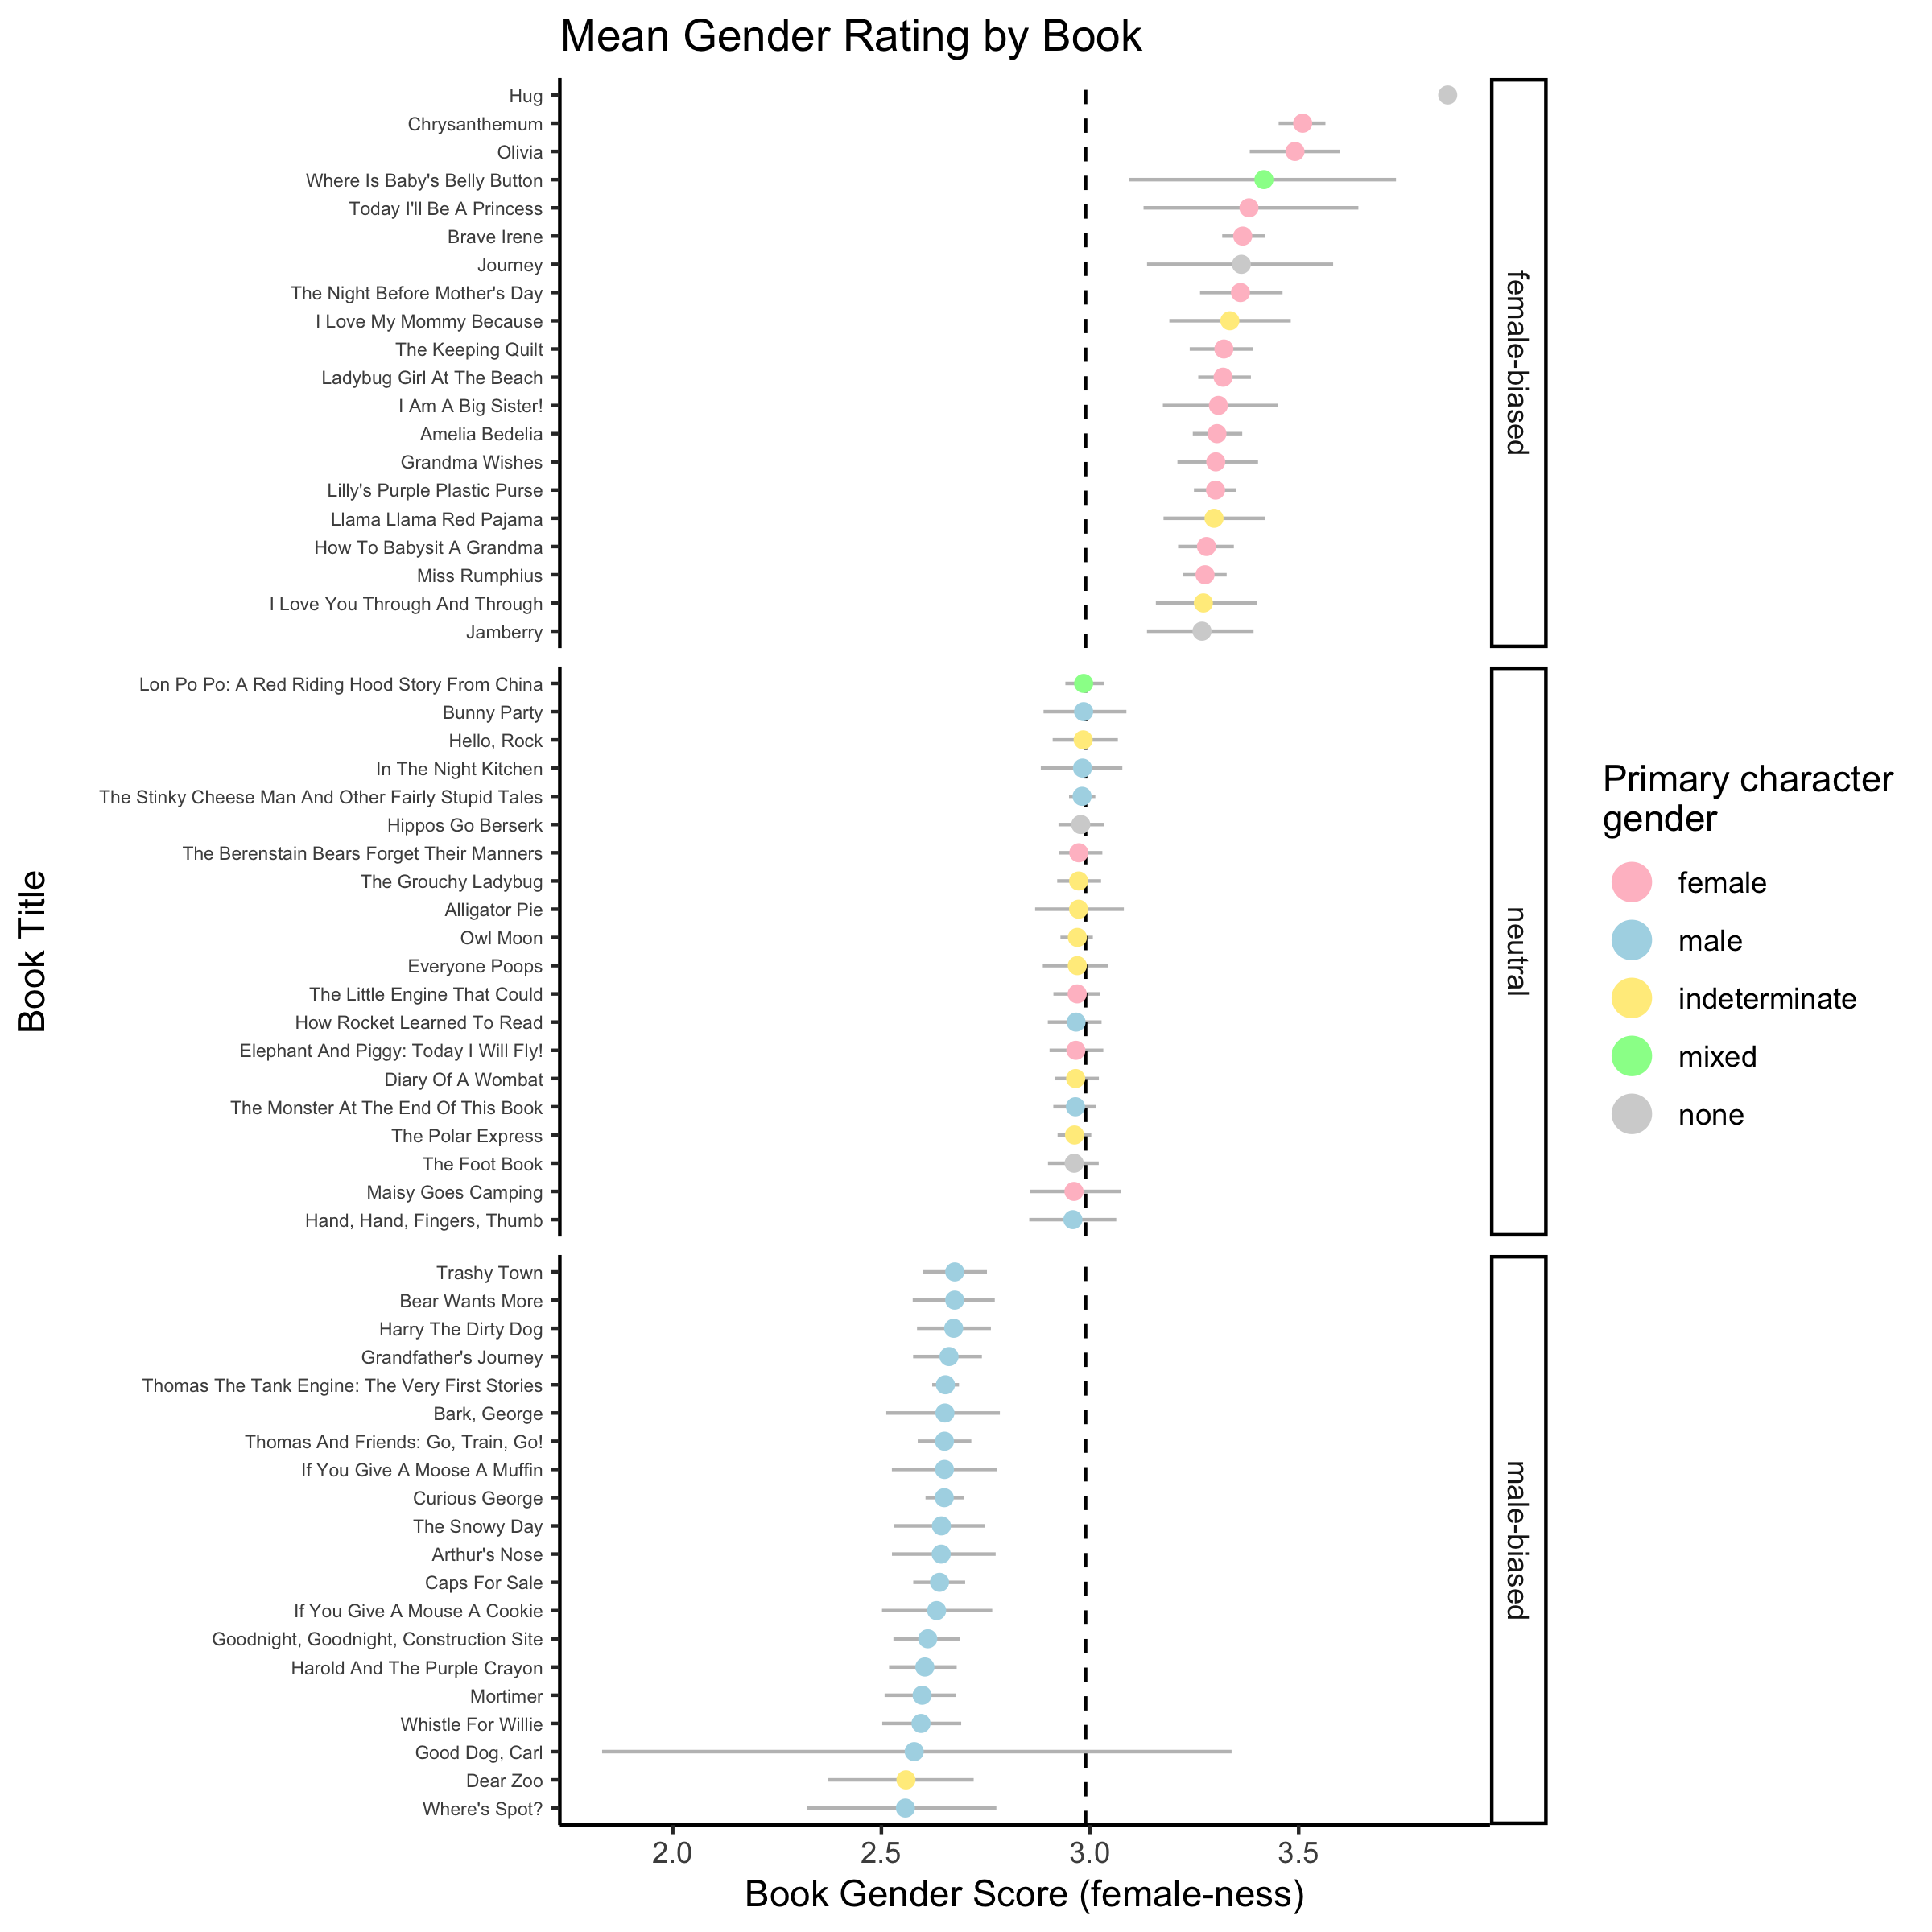
\includegraphics{kidbookgender_psych_sci_files/figure-latex/bookforest-1} \caption{Overall gender rating of  a subset of books, the 20 with the highest feminine bias scores, the 20 with the highest masculine bias scores, and 20 from the neutral range. Bias scores are calculated from the mean gender ratings of words in each book (tokens). The dashed line indicates the overall mean across books, and color indicates the gender of the primary character. Error bars are bootstrapped 95\% CIs.}\label{fig:bookforest}
\end{figure}

\begin{table}

\caption{\label{tab:bookexampletable}Representative female-biased, neutral, and male-biased books}
\centering
\resizebox{\linewidth}{!}{
\begin{threeparttable}
\begin{tabular}[t]{>{\raggedright\arraybackslash}p{4.9em}>{\raggedright\arraybackslash}p{10em}>{\raggedright\arraybackslash}p{10em}>{\raggedright\arraybackslash}p{10em}}
\toprule
\textbf{} & \textbf{female-biased} & \textbf{neutral} & \textbf{male-biased}\\
\midrule
\textbf{Title} & $Chrysanthemum$ & $The\ Polar\ Express$ & $Curious\ George$\\
\addlinespace\addlinespace
\textbf{Main character gender} & female & indeterminate & male\\
\addlinespace\addlinespace
\textbf{Plot summary} & Chrysanthemum is ridiculed at school for her unusual name, despite liking it herself.  She shares her feelings with her parents who console her. After a teacher reveals that she has a similar name, the ridicule stops. & A child travels by train to the North Pole and is gifted a bell from Santa. The bell falls out of the child's pocket on the return home, but is returned as a wrapped present on Christmas morning. & George, a monkey, is taken from his home to the city and repeatedly gets into mischief while exploring his new world. Happily, he eventually is  taken to live at the zoo.\\
\addlinespace\addlinespace
\textbf{Most freq. nouns/ verbs} & chrysanthemum (f), said, name, twinkle (f), father (m), mother (f), flower (f), named (f), thought, way (f), loved (f), school, day, looked, students (f), think (f), chosen, did, tag, would, could (f), grew, morning (f), sounded (f), baby (f) & bell (f), christmas, said, train (m), could (f), elves, express (m), sound, asked, children (f), hear, would, gift (f), lights (f), looked, north (m), pocket, pole (m), silver, stood, bells (f), found, heard, let (f), ringing (f) & man (m), hat (m), hurry, looked, balloon, caught, fire (m), monkey (m), telephone (f), head (m), put, said, saw (f), went (f), bed, catch, ship (m), thought, walked, zoo, do, fireman (m), bag, call, came\\
\bottomrule
\end{tabular}
\begin{tablenotes}[para]
\item \textit{Note: } 
\item  Last row gives 25 most frequent nouns and verbs in each book text. Parentheses denote word gender bias based on human judgments in Study 1a (f = female; m = male).
\end{tablenotes}
\end{threeparttable}}
\end{table}

Overall gender bias could be due to words that express concepts such as ``pretty'' but also the frequency of intrinsically gendered words such as names (e.g., ``Amelia''), pronouns (e.g., ``her''), and relational/generic gender terms (e.g., ``mom,'' ``lady''). We therefore calculated bias separately using intrinsically gendered words referring to characters (the character gender score) and using the remaining content words (content gender score). Character and content scores were moderately correlated (\emph{r} = 0.27 {[}0.13, 0.4{]}, \emph{p} \textless{} .001): books with more gender-biased content tended to have more names, pronouns, and kinship terms of that gender (\autoref{fig:characterplot}a). Thus, the word gender biases reported by adults could arise, in part, from their association with gendered characters.

Whereas the character gender score reflects the extent to which males and females are directly mentioned in a book, the gender of the story protagonist may be particularly salient for children. For each book, we manually coded the name of the primary protagonist character(s) and their gender as determined from text (i.e., pronouns). Text rather than illustrations was used to determine character gender because it was less ambiguous. A character was considered a protagonist if they were the primary agent of the story, in some cases in a collaborative fashion with another protagonist. The main character(s) were classified as either female, male, mixed, or indeterminate (Wagner, 2017). A book was coded as ``mixed'' if there was more than one primary character and their gender composition was heterogeneous, and as ``indeterminate'' if a given primary character had a gender that could not be determined from the text. Two research assistants and the second author coded character gender. Coders agreed on the protagonist type for 97\% of books. Discrepancies were resolved through discussion.

About half of the books (142/247; 57.5\%) had gendered primary characters that were exclusively male or exclusively female. Two-thirds of these books had male primary characters (\emph{N} = 94; \(\chi^2\)(1) = 14.9, \emph{p} \textless{} .001; \emph{d} = 0.68 {[}0.34, 1.03{]}). Of the remaining books, 69 (28\%) had main characters(s) of indeterminate gender, 17 (7\%) had main characters of mixed genders, and 19 (8\%) had no main character(s). These results are broadly consistent with those previously in a smaller sample of books (Wagner, 2017). We then examined book genderedness as a function of the gender of the primary character, using both content and character scores. Books with female primary characters tended to have higher female content scores (\emph{M} = 3.07 {[}3.04, 3.1{]}; \emph{t}(47) = 2.96, \emph{p} = 0.005; \emph{d} = 0.43 {[}0.17, 0.72{]}), compared to the overall averages, whereas books with male primary characters tended to have relatively higher male content scores (\emph{M} = 3 {[}2.98, 3.02{]}; \emph{t}(93) = -2.52, \emph{p} = 0.01; \emph{d} = -0.26 {[}-0.5, -0.05{]}; \autoref{fig:characterplot}b). This difference, albeit small in an absolute sense, exists even taking the grand average of the genderedness of words across the entire book. Notably, however, there was a large degree of variability in content scores across books (female: \(SD\) = 0.72; male: \(SD\) = 0.69): many books with male characters had female-biased content-words and vice-versa. Finally, there was a trend for more recently published books to have proportionally fewer male main characters, and more main characters with indeterminate gender (\autoref{fig:historicalplot}; see SI for additional analyses).

\begin{figure}[t!]
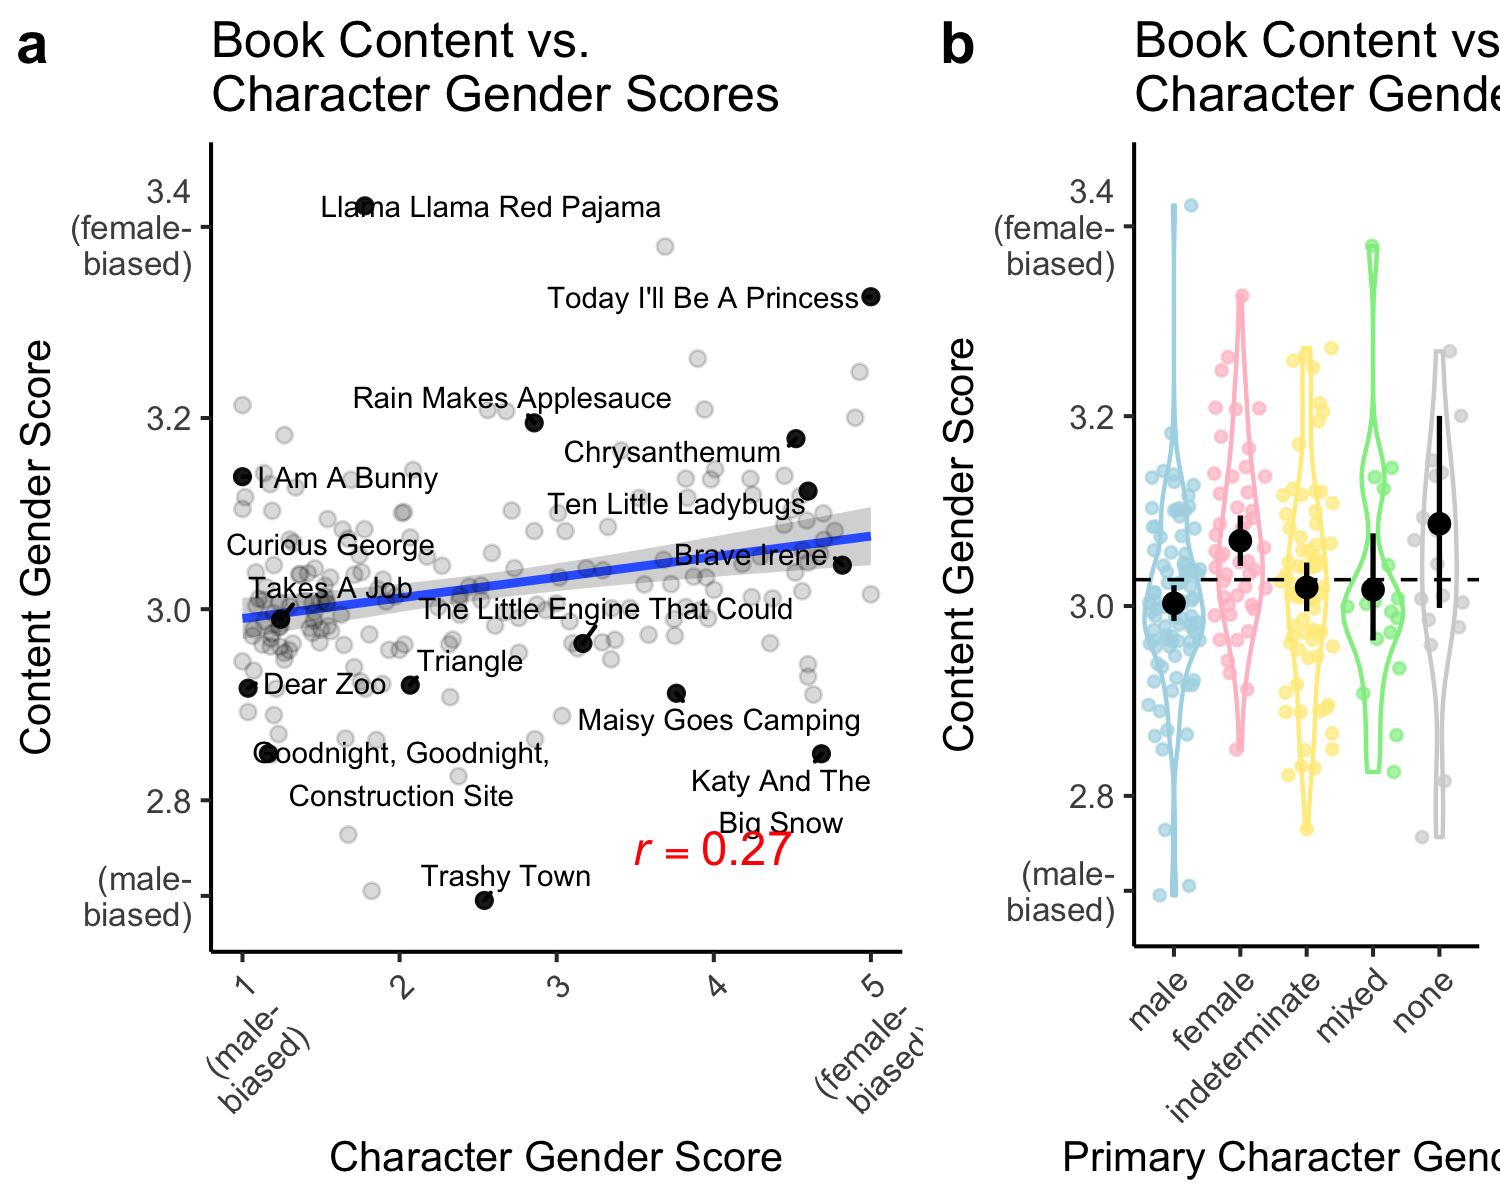
\includegraphics[width=\textwidth,]{kidbookgender_psych_sci_files/figure-latex/characterplot-1} \caption{(a) Mean content gender score for each book as a function of mean character gender score. Error bar shows the standard error of the linear model fit.  (b) Distribution across books of content gender score as a function of primary character gender. Colored points show individuals books (one point excluded for visibility). Dashed line shows content gender score grand mean. Black points and error bars show mean and bootstrapped 95\% percent confidence intervals for books of each primary character gender type.}\label{fig:characterplot}
\end{figure}

\begin{figure}[t!]
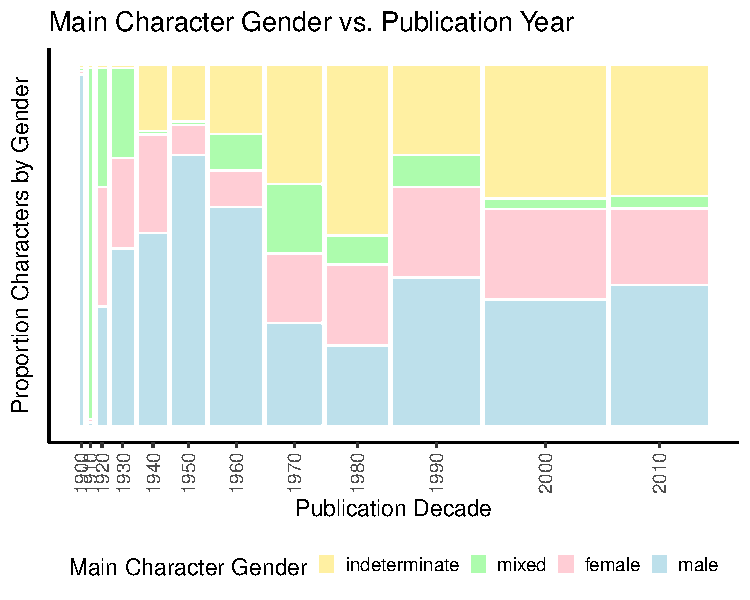
\includegraphics{kidbookgender_psych_sci_files/figure-latex/historicalplot-1} \caption{The proportion of books with main characters in each gender category (male, female, mixed and indeterminate) as a function of publication year. Bar width corresponds to the number of books in the WCBC corpus published in each decade.}\label{fig:historicalplot}
\end{figure}

Our findings suggest that books vary considerably along gender not only in terms of characters (i.e., those having only male or only female characters), which is expected, but also in terms of gendered content words. Books with female characters tend to have content (e.g., artifacts, actions, descriptors) that is more associated with females, whereas books with male characters tend to have content on average more associated with male, though this effect is highly variable across books.

\hypertarget{study-1c-validation-of-book-gender-bias-measure}{%
\subsection{Study 1c: Validation of book gender bias measure}\label{study-1c-validation-of-book-gender-bias-measure}}

We estimated each book's gender bias using a simple average of the gender bias of the words comprising them. Of course, the words actually occur in contexts that could modulate their bias. For example, the gender bias of ``brave'' would be the same whether it occurred in the sentence ``Sally is brave'' or ``Sally is not brave.'' To address this concern, we asked a new group of adult participants to provide information about main characters after reading the complete text of a book. We could then determine whether these participant-generated descriptions exhibited the gender biases identified using the simpler word-based measure. The two should diverge if book genderedness as estimated by averaging isolated words is unrepresentative of the story context.

\hypertarget{method-2}{%
\subsubsection{Method}\label{method-2}}

We recruited 152 participants from Amazon Mechanical Turk. Eighty-one identified as female, 65 identified as male, 6 did not provide a response.

We divided the books in our corpus into quintiles based on the average gender score described in Study 1b, and selected 15 books each from the first (female-biased: \emph{M} = 3.23; \emph{SD} = 0.06), third (neutral: \emph{M} = 2.96; \emph{SD} = 0.03), and fifth quintiles (male-biased: \emph{M} = 2.64; \emph{SD} = 0.03) to be evaluated. We excluded books that were either very short or very long (less than 100 words, or more than 900 words), or those without a gendered main character.

Participants were presented with the complete text of a book, and told that they would be asked questions about the characters in it. After reading the text, participants were asked to list 2-5 main activities of a specified character (e.g., ``List 2-5 main activities \emph{Thomas} does in the story.''). The full text of the book was displayed on the same page so that participants did not have to rely on memory to answer the question. Next, participants were asked to complete a similar procedure but provide descriptions of the character's traits (e.g., ``List 2-5 words to describe \emph{Thomas} in the story.''). This procedure was repeated for all main and secondary characters in a book. Each participant provided responses for both character activities and character traits for three books.

On average, participants generated 3.83 responses per question (\emph{SD} = 1.24). Responses were lemmatized, corrected for spelling, and, in cases where a multi-word phrase was listed (e.g., ``builds a castle''), the first word was selected for analysis. We identified the part of speech for the first word and excluded responses of the wrong class, analyzing only verbs for the activity question and adjectives, adverbs, and nouns for the trait question. We also excluded responses that were very long (more than 35 characters), as these were likely to be full sentences rather than activity or trait words. In total, 4\% of responses were excluded, leading to a final sample of 4,889 responses and 947 unique lemmas. We then analyzed the gender bias of the activity and trait words using previously-collected human judgments of word gender bias, which covered 67\% of the word tokens used to describe characters and their activities. We collected an additional set of human judgments (\emph{N} = 251; \emph{M} = 11.33 ratings/word; \emph{SD} = 0.95) such that gender bias estimates were available for all words produced more than once in Study 1c (93\% of tokens; see SI).

\hypertarget{results-1}{%
\subsubsection{Results}\label{results-1}}

\begin{figure}[t]
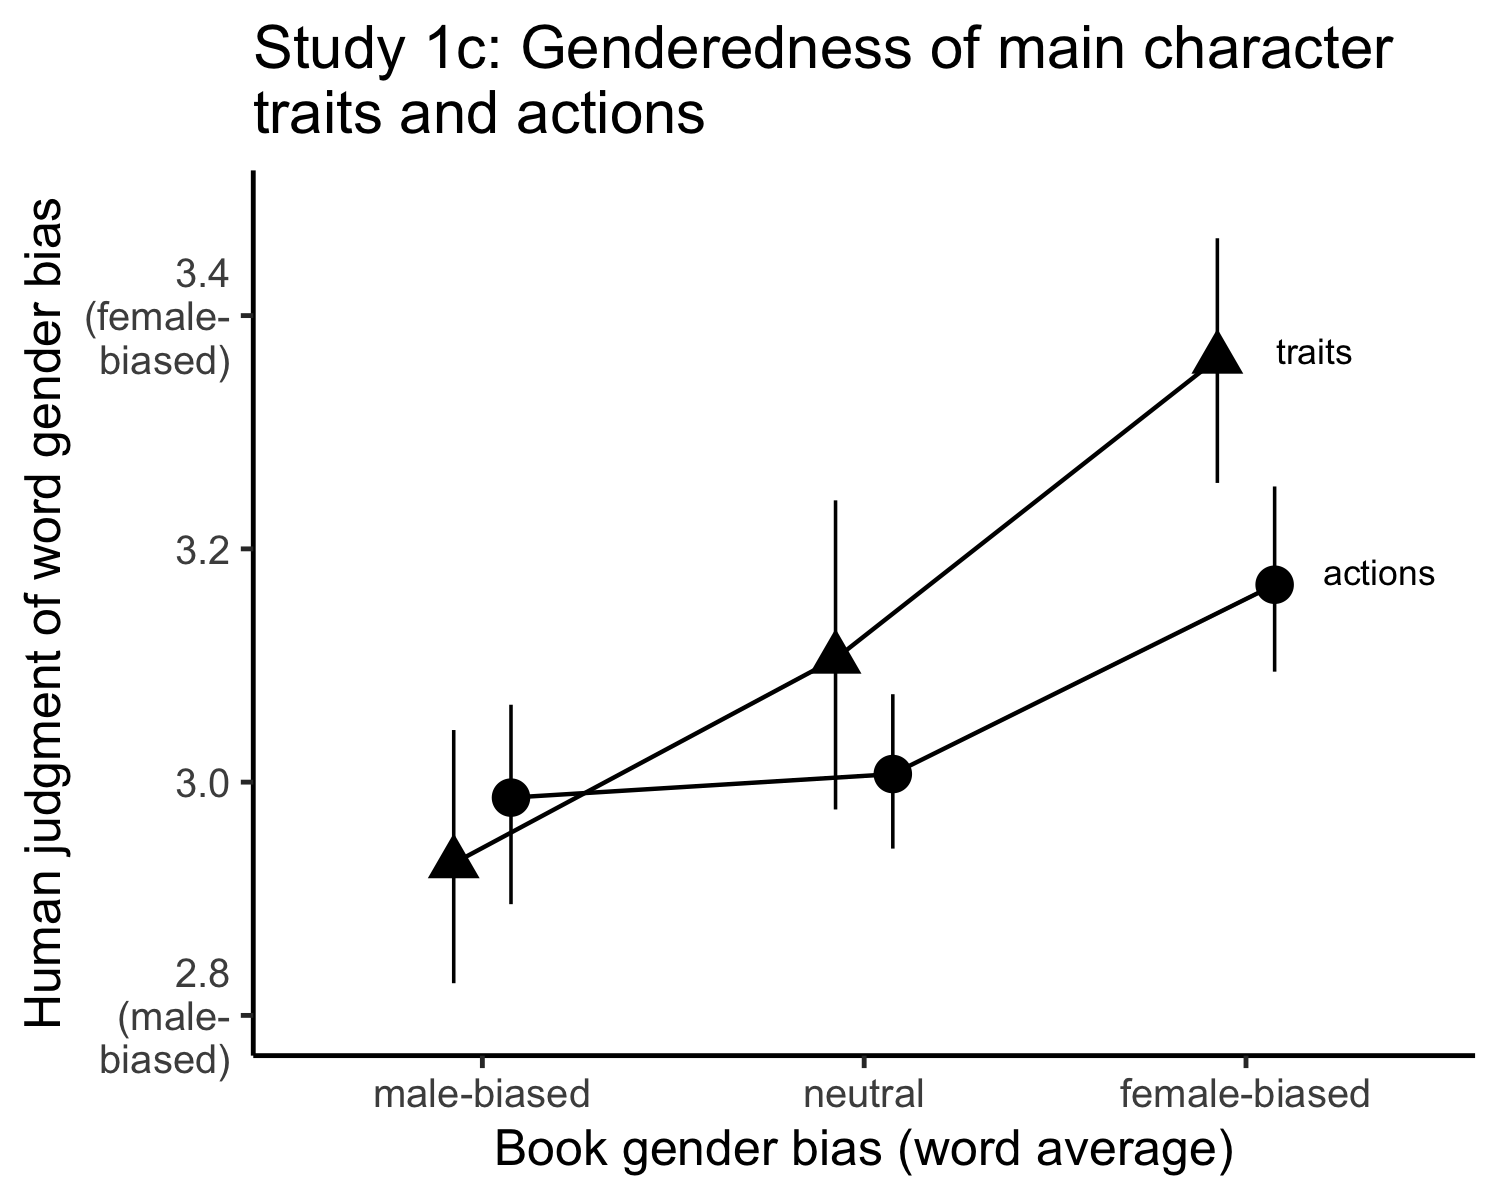
\includegraphics{kidbookgender_psych_sci_files/figure-latex/validationplot-1} \caption{Average genderedness of words generated in Study 1c to describe the main character's traits (triangles) and actions (circles). Error bars are bootstrapped 95\% CIs.}\label{fig:validationplot}
\end{figure}

The main question is whether the descriptions of book characters' traits and their actions generated by participants who read the books exhibited the same gender biases derived by averaging the gender scores for words in the texts. We fit mixed-effect linear regression models predicting the gender biases of characters' traits and actions from the averaged word gender of a book. The averaged word gender of a book was treated as a continuous fixed effect, and book and participant were included as random intercepts. The averaged word gender of a book predicted the gender bias of both the activity (\(\beta\) = 0.13; \emph{SE} = 0.05; \emph{t} = 2.74) and trait words generated by participants (\(\beta\) = 0.24; \emph{SE} = 0.05; \emph{t} = 5.12; \autoref{fig:validationplot}). Averaged word gender based on exclusively content words predicted activity (\(\beta\) = 0.22; \emph{SE} = 0.04; \emph{t} = 5.43) and trait words (\(\beta\) = 0.21; \emph{SE} = 0.05; \emph{t} = 4.42) to a similar extent, whereas averaged word gender based on exclusively character words predicted trait words (\(\beta\) = 0.21; \emph{SE} = 0.05; \emph{t} = 4.01) but not activity words (\(\beta\) = 0.05; \emph{SE} = 0.05; \emph{t} = 1.07; see SI for full model results). These results suggest that the averaged word gender measure described in Study 1b captures aspects of book gender bias, even after taking into account the broader context of the book text. Further, the difference in the genderedness of traits associated with by male vs.~female primary characters is substantially larger than the effect observed in Study 1b. For example, male characters were more than twice as likely as female characters to be described as ``playful'' or ``fun,'' whereas female characters were more than twice as likely as male characters to be described as ``caring'' or ``quiet.''

\hypertarget{study-2-measuring-gender-bias-through-co-occurrence-statistics}{%
\section{Study 2: Measuring gender bias through co-occurrence statistics}\label{study-2-measuring-gender-bias-through-co-occurrence-statistics}}

So far we have presented findings about gendered information in children's books based on adult gender norms and semantic representations derived from adult text. The results are relevant to the beliefs of adults who read books with children, which they may convey during shared reading. In this study we sought to measure genderedness independently of adult ratings. To do this, we trained word embedding models on the full text of the WCBC. Despite the smaller size of the children's book corpus, the word embeddings yield coherent patterns and clear evidence for gender biases similar to those identified from adult texts and norms. Overall, children's books exhibited stronger gender stereotypes than comparable adult texts.

\hypertarget{study-2a-word-gender-associations-in-the-childrens-book-corpus}{%
\subsection{Study 2a: Word gender associations in the Children's Book Corpus}\label{study-2a-word-gender-associations-in-the-childrens-book-corpus}}

\hypertarget{method-and-results-1}{%
\subsubsection{Method and Results}\label{method-and-results-1}}

A word embedding model was trained on the full corpus of text from all 247 books (see SI for training details). We then estimated the gender association for each word by calculating its mean semantic similarity (cosine distance) to a set of unambiguously female anchor words (``woman,'' ``girl,'' ``sister,'' ``she,'' ``her,'' and ``daughter''), and a corresponding set of male words ({``man,''} {``boy,''} {``brother,''} {``he,''} {``him,''} and {``son,''} Caliskan, Bryson, \& Narayanan, 2017; Lewis \& Lupyan, 2020). A female gender score was calculated for each word as the mean female similarity minus the mean male similarity. For comparison, we also estimated these scores from models trained on an identically sized corpus of adult fiction published from 1990 to 2017 (Davies, 2008), and a much larger corpus of Wikipedia (Bojanowski, Grave, Joulin, \& Mikolov, 2016). We then examined how these estimates of word gender bias derived from language statistics compared to the gender norms we had previously collected from participants.

There were 1,893 words common across the word embedding models and human gender norms dataset. Estimates of word-embedding gender bias from the WCBC were correlated with adult judgments of word bias (\emph{r} = 0.27 {[}0.23, 0.31{]}, \emph{p} \textless{} .001): Words that adult participants rated as more feminine (or masculine) tended to be similarly biased in the language statistics of the WCBC. Estimates of gender bias from the WCBC were also correlated with word-embedding gender bias from a model trained on adult fiction (\emph{r} = 0.36 {[}0.32, 0.4{]}, \emph{p} \textless{} .001), as well as the model trained on Wikipedia (\emph{r} = 0.32 {[}0.28, 0.36{]}, \emph{p} \textless{} .001; see SI for all pairwise correlations). The moderate size of these correlations is likely due in part to the relatively small size of the WCBC corpus, as this relationship tends to be much larger in larger corpora (cf.~Lewis \& Lupyan, 2020).

These findings suggest that some of the word-level gender associations that emerge in adulthood begin to appear in the statistics of children's texts, and could be potentially learnable from exposure to children's books.

\hypertarget{study-2b-specific-gender-stereotypes-in-childrens-books}{%
\subsection{Study 2b: Specific gender stereotypes in children's books}\label{study-2b-specific-gender-stereotypes-in-childrens-books}}

We next examined gender bias beyond the word level, asking whether children's books instantiate specific gender stereotypes.

\hypertarget{method-and-results-2}{%
\subsubsection{Method and Results}\label{method-and-results-2}}

We focused on four gender stereotypes seen in studies of adults and children: (1) Women as ``good,'' men as ``bad''; (2) Women as better at language skills, men as better at math skills; (3) Women as better at art skills, men as better at math skills, and (4) Women as family-oriented, men as career-oriented. Each of these stereotypes has been demonstrated in behavioral studies using both explicit measures (e.g., asking ``How strongly do you associate career and family with males and females?'') and implicit measures, such as the Implicit Association Test (IAT; Greenwald, McGhee, and Schwartz, 1998; \autoref{tab:iattable}). The IAT quantifies these associations using reaction time in a word categorization task (e.g., women-good, men-bad vs.~women-bad, men-good), though not without criticism about its validity (Greenwald et al., 2020; Oswald, Mitchell, Blanton, Jaccard, \& Tetlock, 2013). Faster responses are taken to indicate that two categories are more closely cognitively associated.

The biases found in the IAT are also present in the distributional semantics of language (Caliskan, Bryson, \& Narayanan, 2017; Lewis \& Lupyan, 2020). A bias can be quantified in a word embedding model as an effect size, using the same set of word items as in the behavioral IAT. The effect size is calculated as the relative (cosine) similarity of male words (e.g., ``men'') to male-stereotyped words (e.g., ``work''), compared to the relative similarity of female words (e.g., ``women'') to female-stereotyped words (e.g., ``family''; see SI for formal effect size description). Stereotypes that are revealed in the IAT as measured by reaction time (e.g., men-work; women-family) tend to be reflected in word embedding models, as measured by cosine distance.

We used this method to examine whether the four gender-related biases are also present in the language statistics of the WCBC. Target category items are listed in \autoref{tab:iattable}, along with references for the corresponding IAT experiments with children and adults. Gender category word items were identical to those used in Study 2a. Other items were taken from the corresponding behavioral experiments, replacing items with more child-friendly alternatives in cases where the target word did not occur in the WCBC (e.g., ``algebra'' was changed to ``numbers''). We conducted this analysis on a model trained on the WCBC, as well as models trained on a sample of the adult fiction matched in size to the WCBC (Davies, 2008) and a model trained on Wikipedia (Bojanowski, Grave, Joulin, \& Mikolov, 2016). The starting point for the text from the adult fiction book was randomly determined. We trained 10 models each on the COCA and WCBC corpora and estimated the average effect size for each IAT type.

\begingroup\fontsize{9}{11}\selectfont

\begin{ThreePartTable}
\begin{TableNotes}[para]
\item \textit{Note:} 
\item The left column describes the bias; the middle column lists the actual words tested for the target categories; the right column cites behavioral studies measuring the psychological bias. The words for the ``female" and ``male" categories were identical across all tests (see Main Text). Note that the words differ slightly from the stimuli used in the behavioral studies. ``C" and ``A" in citations indicate whether  participants were children or adults, respectively.
\end{TableNotes}
\begin{longtabu} to \linewidth {>{\raggedright\arraybackslash}p{9em}>{\raggedright\arraybackslash}p{27em}>{\raggedright\arraybackslash}p{15em}}
\caption{\label{tab:iattable}Four IATs used to study gender bias}\\
\toprule
Psychological Bias & Target Words & Behavioral Studies\\
\midrule
women as good;\newline men as bad & ``good": good, happy, gift,  sunshine, heaven\newline ``bad": bad, awful, sick, trouble, hurt & Cveneck, Meltzoff, \& Greenwald (2011b, C); Skowronski \& Lawrence (2001, C/A); Greenwald et al. (2002, A); Rudman \& Goodman (2004, A)\\
\addlinespace\addlinespace
women and family;\newline men and career & ``family": family, parents, children, home, cousins, wedding\newline ``career": job,  work,  money, office, business, desk & Nosek, Banaji,   \& Greenwald (2002, A)\\
\addlinespace\addlinespace
women and language;\newline men and math & ``language": books, read, write, story, letters, spell\newline ``math": numbers, count,  sort,  size, shapes, different & Cveneck, Meltzoff, Greenwald (2011a, C); Nosek, Banaji,  \& Greenwald, (2002, A)\\
\addlinespace\addlinespace
women and arts;\newline  men and math & ``art": art, paint, draw, books, dance, story\newline ``math": numbers, count,  sort,  size, shapes, different & Nosek, Banaji \& Greenwald (2002, A)\\
\bottomrule
\insertTableNotes
\end{longtabu}
\end{ThreePartTable}
\endgroup{}

\begin{figure}[t!]
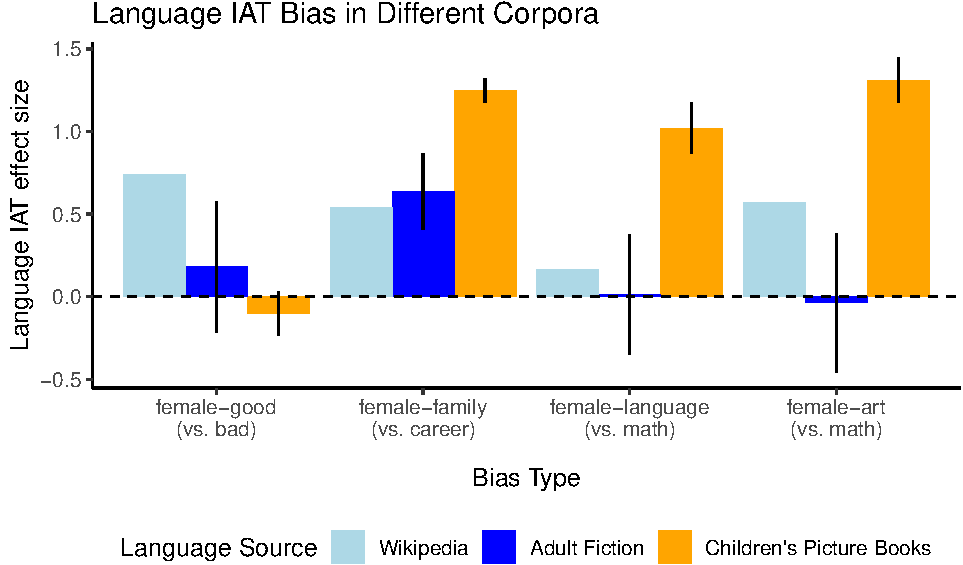
\includegraphics[width=\textwidth,]{kidbookgender_psych_sci_files/figure-latex/languageiat-1} \caption{Estimates of the magnitude of gender biases in word embedding models trained on the Wisconsin Children’s Book Corpus (orange), adult fiction corpus (COCA; dark blue), and Wikipedia (light blue). Positive effect sizes indicate a bias to associate women with the stereotypical category (e.g., ‘family'); negative effect sizes indicate a bias to associate women with the non-stereotypical category (e.g., ‘career’).  Ranges indicate 95\% confidence intervals across models. Biases are described more fully in Table 3.}\label{fig:languageiat}
\end{figure}

\autoref{fig:languageiat} shows the effect size for each of the four biases from models trained on each of the three corpora. Positive values indicate a bias to associate women with the stereotypical female category (e.g.~women-family). Three of the four gender biases were present in the co-occurrence statistics of the WCBC -- Language-Math, Arts-Math, and Family-Career. Importantly, these biases were larger in children's books than in corpora containing mostly adult-directed language. This finding that behaviorally measurable gender biases are present in an exaggerated form in books for young children provides additional evidence that these books instantiate gender stereotypes that may influence children's learning of gender stereotypes.

In summary, these studies show that both adult word gender associations and specific gender stereotypes observed in behavioral studies with adults and children are reflected in the co-occurrence statistics of the children's book corpus. These findings are consonant with prior work showing similar biases in a historical corpus of children's books published around 1900 (Charlesworth, Yang, Mann, Kurdi, \& Banaji, 2021),

\hypertarget{study-3-book-gender-and-child-gender}{%
\section{Study 3: Book gender and child gender}\label{study-3-book-gender-and-child-gender}}

The results so far suggest that the texts of popular children's books contain rich information about gender. In this final study, we sought to better understand the processes through which this information might influence children's socialization into gender stereotypes by examining who is being exposed to these books. We created a novel measure based on the content of book reviews on a large online bookstore and validated this measure using existing survey data directly measuring the audience of a book. These data indicate that children's books more frequently read to girls tend to have both more female content and more female characters, and children's books more frequently read to boys tend to have both more male content and more male characters.

\hypertarget{method-3}{%
\subsubsection{Method}\label{method-3}}

For each book in the WCBC we collected a sample of the most recent reviews on Amazon.com. There were reviews for all but two books, with an average of 473.96 reviews per book (\emph{SD} = 194.53; min = 1; max = 1,290). The content of each review was coded for the presence of 16 gendered kinship terms (e.g., ``son,'' ``daughter,'' ``nephew,'' ``niece''; see SI for full list). We selected these target words because they had a high likelihood of referring to the child for whom the book was purchased (e.g., ``My son loves \emph{Goodnight Moon}.''), rather than referring to a book character. All but two books had reviews containing at least one of our target gendered kinship terms. Overall, 27.6\% of reviews per book contained at least one target gendered kinship term (\emph{SD} = 0.08). For each review, we calculated an audience gender score as the proportion of female kinship terms (tokens) present relative to all target kinship words, and then averaged across reviews from the same book to get a book-level estimate of the gender of book addressees (\emph{M} = 0.49; \emph{SD} = 0.19; see SI for supplemental models predicting book gender at the review level).

We validated our computed audience gender score by comparing it to survey data collected by Hudson Kam and Matthewson (2017), who asked a sample of 1,107 Canadian caregivers to list the five books most frequently read to their male or female child. Of the books with at least 5 survey responses, 103 were also in the WCBC. Our review-based gender measure was positively correlated with Hudson Kam and Matthewson's survey based measure (\emph{r} = 0.58 {[}0.44, 0.7{]}, \emph{p} \textless{} .001), suggesting that book reviews can be used to estimate whether a given book is primarily read to boys or girls.

\hypertarget{results-2}{%
\subsubsection{Results}\label{results-2}}

\begin{figure}[t!]
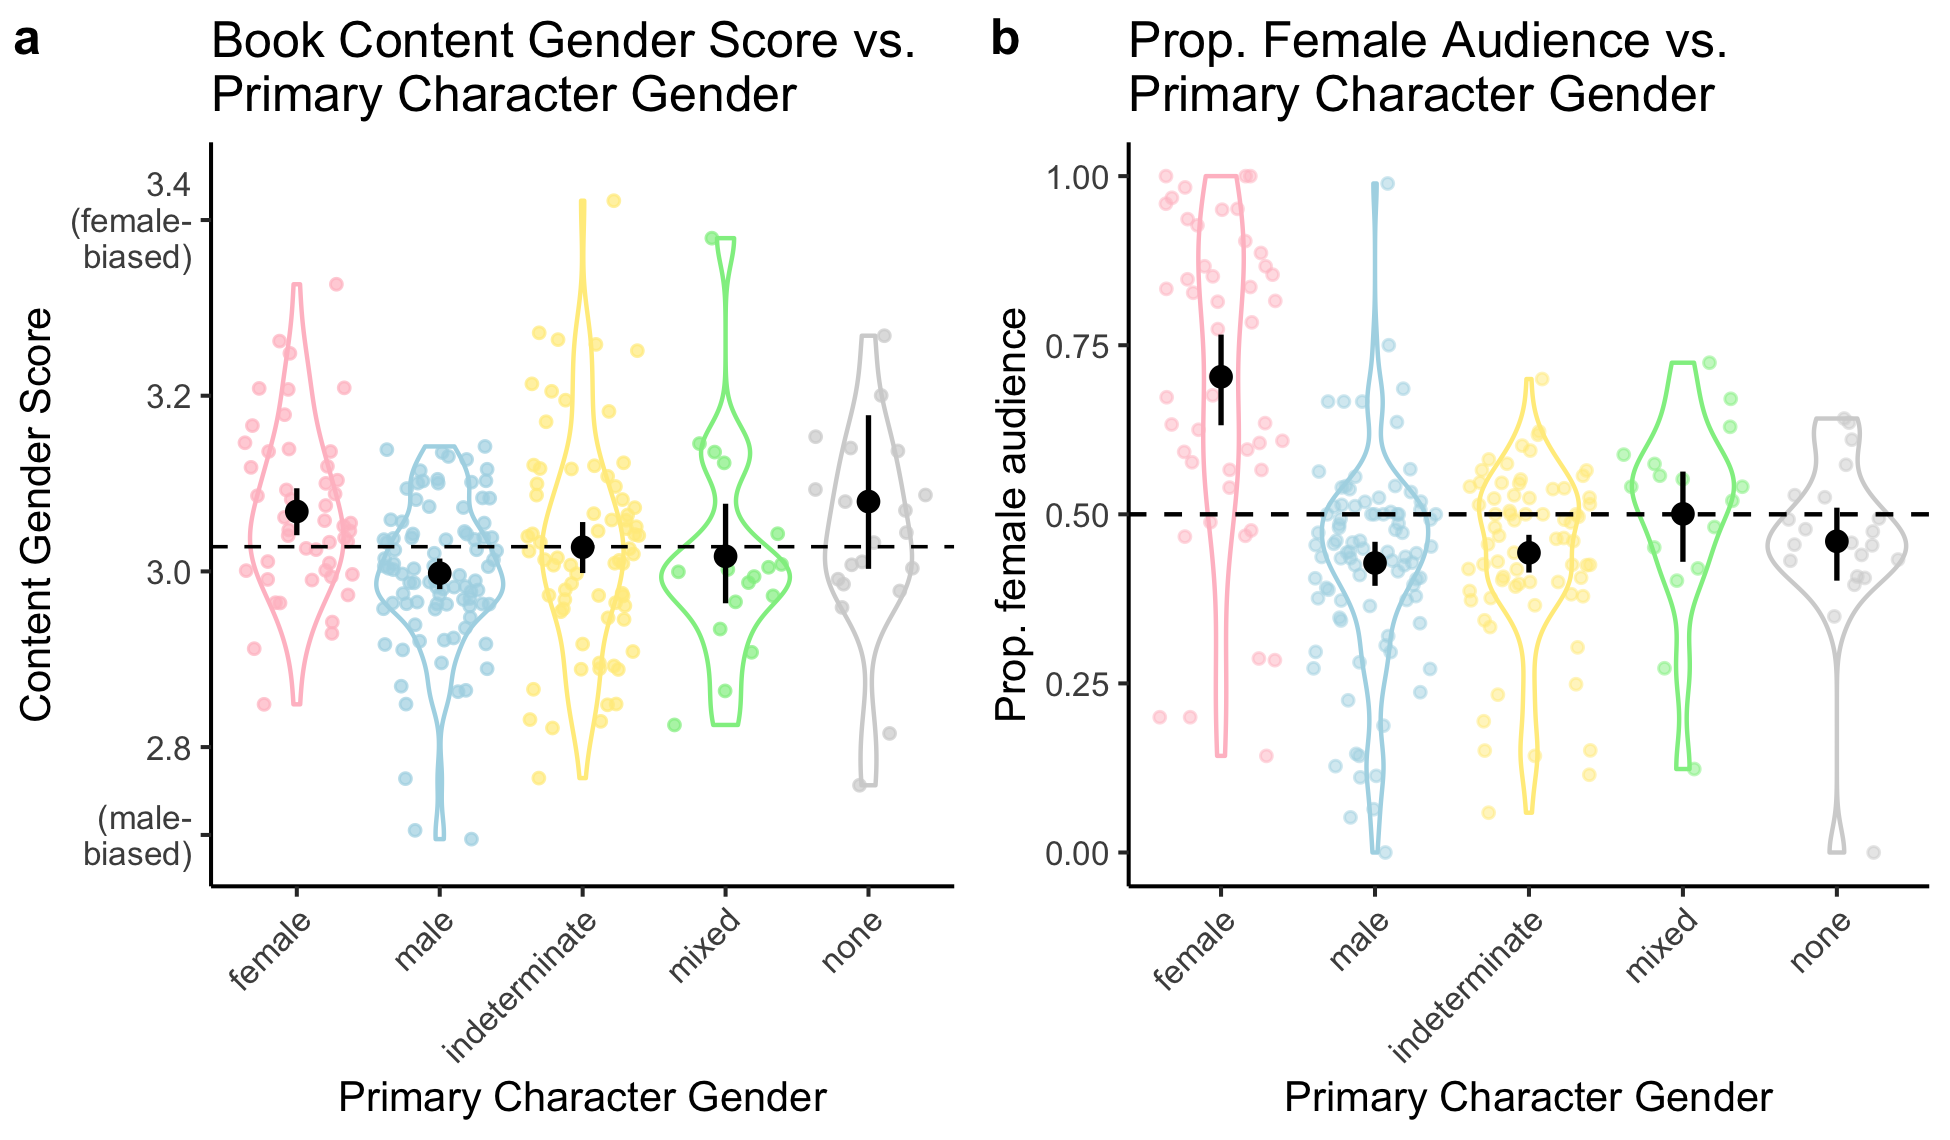
\includegraphics[width=\textwidth,]{kidbookgender_psych_sci_files/figure-latex/characterplots-1} \caption{(a) Estimated audience gender for each book as a function of mean character gender score. Error bar shows the standard error of the linear model fit. (b) Distribution across books of audience gender as a function of primary character gender. Colored points show individuals books. Dashed line shows grand mean of proportion female audience. Black points and error bars show mean and bootstrapped 95\% percent confidence intervals for books of each primary character gender type.}\label{fig:characterplots}
\end{figure}

We compared our audience gender score for each book to the measures of book genderedness described above. Both the content gender scores (\emph{r} = 0.37 {[}0.26, 0.48{]}, \emph{p} \textless{} .001) and book character gender scores (\emph{r} = 0.53 {[}0.41, 0.62{]}, \emph{p} \textless{} .001; \autoref{fig:characterplots}a) were correlated with audience gender scores: Books that contained more female-biased content words and more female characters tended to be read more often to girls. In an additive linear model predicting audience gender with both types of gender scores, both content (\(\beta\) = 0.67; \emph{SE} = 0.12; \emph{Z} = 5.47; \emph{p} \textless{} .001) and character gender scores (\(\beta\) = 0.07; \emph{SE} = 0.01; \emph{Z} = 7.32; \emph{p} \textless{} .001) predicted independent, and roughly equal, variance. Together, they accounted for 37\% of the total variance in audience gender.

Consistent with this general pattern, books with female primary characters also tended to be more often read to girls, compared to the overall average (\emph{t}(46) = 7.04, \emph{p} \textless{} .001; \emph{d} = 1.03 {[}0.68, 1.53{]}; \autoref{fig:characterplots}b). Books with male (\emph{t}(92) = -5.08, \emph{p} \textless{} .001; \emph{d} = -0.53 {[}-0.72, -0.35{]}) or gender indeterminate primary characters (\emph{t}(68) = -3.2, \emph{p} = 0.002; \emph{d} = -0.39 {[}-0.58, -0.18{]}) tended to be more often read to boys. Notably, the effect size for girls was more than twice that of boys, suggesting that there was a stronger bias to read books with female characters to girls, relative to books with male characters to boys. There was no bias in audience gender for books with multiple primary characters of different genders (\emph{t}(16) = 0.26, \emph{p} = 0.8; \emph{d} = 0.06 {[}-0.36, 0.83{]}) or books without primary characters (\emph{t}(18) = -1.03, \emph{p} = 0.32; \emph{d} = -0.24 {[}-0.94, 0.2{]}).

In sum, these findings suggest that children's books featuring a particular gender and content associated with that gender tend to be read disproportionately to children of that gender.

\hypertarget{general-discussion}{%
\section{General Discussion}\label{general-discussion}}

What gender messages are conveyed by popular children's books and who is being exposed to them? We constructed a corpus of 247 contemporary children's books and analyzed the extent to which the books contain biased gender associations. Using adult judgments of individual words, we found that over half of the words in the corpus tended to be associated with a particular gender, and tended to cohere in gender stereotypical categories. At the book level, we found that books varied in their gender associations, and that the associations tended to reflect gender stereotypes (e.g., girl characters tended to do stereotypically girl activities). Further, the language statistics of the corpus itself paralleled word gender biases seen in adult judgments and specific gender stereotypes (e.g., boys are better at math, and girls are better at reading). These biases were more exaggerated in the children's book corpus, relative to adult fiction. Finally, we derived a novel metric for measuring the gender distribution of a book's audience using automated analysis of book reviews. Children tended to be exposed to books that conveyed gender stereotypes about their own gender. Our work provides the first quantitative assessment of how gender is represented in contemporary children's books and reveals that they contain many statistical regularities that could inform children's development of gender stereotypes.

A notable pattern across our results is that female biases tend to be larger than male biases. In Study 1, books tended to have content that was biased toward the gender of the primary character (books with female characters have female content; books with male characters have male content), but this effect was larger for female characters than male characters. Similarly, participants tended to associate male characters with gender-neutral actions and traits, but female characters with female-biased actions and traits. This tendency was also seen in the audience of books: girls were far more likely to be read a book with a female primary character than boys were to be read a book with a male primary character. One interpretation of this general pattern is that ``male'' is conceptualized as the default, unmarked gender. This is consistent with the tendency for languages to treat male as the unmarked gender in their morphology (e.g., the word ``female'' is derived from adding a prefix to ``male''), as well as numerous other empirical phenomena (e.g., Johns \& Dye, 2019).

There are several reasons to think that the statistical regularities we identified in children's books may be shaping children's gender stereotypes. First, many of the stereotypical patterns that we report are implicit in text statistics, rather than conveyed via explicit statements (``boys are better at math than girls''). The implicit nature of these messages may make them particularly difficult for adult readers to track or explicitly contradict. Second, children are exposed to books with a caregiver (more often than, e.g., watching TV). The caregiver's presence may signal implicit endorsement of these stereotypes as correct or desirable and lead the child to make stronger inferences (Lewis \& Frank, 2016; Xu \& Tenenbaum, 2007). Third, our data suggest that children tend to be exposed to books that contain own-gender-consistent associations. This may make gender-inconsistent preferences less familiar to children and therefore more difficult to emulate (Bussey \& Bandura, 1999). Filtered through children's cognitive and social biases, children's books may therefore be a potent means of teaching children about gender stereotypes.

One unanswered question from our data is how children learn stereotypes about other genders, given that they are largely read storybooks containing stereotypes aligning with their own gender. One possibility is that children gain information about other genders from other sources, such as media and direct interactions. Alternatively, children may in fact receive more information about their own gender, than about others, and consequently have less precise intuitions about stereotypes related to other genders. It is also an open question whether the tendency for children to be read books matching their own gender is due to caregiver or child preferences. This question is important in light of recent data on gender development in transgender children who show strong identity with the gender they feel they are by age three (Gülgöz et al., 2019). If transgender children play an active role in their own socialization (Martin \& Ruble, 2004), our data suggest that children's books could be an early source of gender information for them.

Our work characterizes the gendered content of children's books and their potential role in development, but causal links between the properties we observed and the gender associations that children form remain to be addressed. Reviews of the impact of shared reading on language and literacy development have concluded that learning effects are small (Noble et al., 2019; Scarborough \& Dobrich, 1994). How much is learned about gender in particular is a further question. Moreover, little is known about how children themselves perceive the messages contained within these books. In the work presented here, we primarily measure word gender bias via adult judgments, yet children do not have the extensive knowledge and experience that underlies adult judgments. The fact that word embedding models trained exclusively on the statistics of the children's book corpus reflect adult-like word gender biases suggests that adult gender biases could in principle begin to be learned from children's book texts, but whether they are remains an open question. Future work could more directly address these questions by eliciting child judgments of word gender, and by experimentally manipulating the statistics of children's linguistic input about gender.

There is no doubt that shared reading has numerous benefits. However, our data show that contemporary children's books also convey systematic information about gender, often (though not always) instantiating gender stereotypes --- indeed some more strongly than in adult-directed literature. Caregivers may inadvertently promote the development of gender stereotypes via shared reading of books. Exposure to these language-embedded biases may lead to beliefs that help entrench gender biases and disparities. However, the variability of gender biases across books also suggests that caregivers may be able to influence children's development of beliefs about gender through choice of books, an important issue for future research.

\newpage

\hypertarget{references}{%
\section{References}\label{references}}

\setlength{\parindent}{-0.5in}
\setlength{\leftskip}{0.5in}

\hypertarget{refs}{}
\begin{CSLReferences}{1}{0}
\leavevmode\hypertarget{ref-bian2017gender}{}%
Bian, L., Leslie, S.-J., \& Cimpian, A. (2017). Gender stereotypes about intellectual ability emerge early and influence children's interests. \emph{Science}, \emph{355}(6323), 389--391.

\leavevmode\hypertarget{ref-bojanowski2016enriching}{}%
Bojanowski, P., Grave, E., Joulin, A., \& Mikolov, T. (2016). Enriching word vectors with subword information. \emph{arXiv Preprint arXiv:1607.01759}.

\leavevmode\hypertarget{ref-bus1995joint}{}%
Bus, A. G., Van Ijzendoorn, M. H., \& Pellegrini, A. D. (1995). Joint book reading makes for success in learning to read: A meta-analysis on intergenerational transmission of literacy. \emph{Review of Educational Research}, \emph{65}(1), 1--21.

\leavevmode\hypertarget{ref-bussey1999social}{}%
Bussey, K., \& Bandura, A. (1999). Social cognitive theory of gender development and differentiation. \emph{Psychological Review}, \emph{106}(4), 676.

\leavevmode\hypertarget{ref-caliskan2017semantics}{}%
Caliskan, A., Bryson, J. J., \& Narayanan, A. (2017). Semantics derived automatically from language corpora contain human-like biases. \emph{Science}, \emph{356}(6334), 183--186.

\leavevmode\hypertarget{ref-charlesworth2021gender}{}%
Charlesworth, T. E., Yang, V., Mann, T. C., Kurdi, B., \& Banaji, M. R. (2021). Gender stereotypes in natural language: Word embeddings show robust consistency across child and adult language corpora of more than 65 million words. \emph{Psychological Science}, \emph{32}(2), 218--240.

\leavevmode\hypertarget{ref-chen2017evaluating}{}%
Chen, D., Peterson, J. C., \& Griffiths, T. L. (2017). Evaluating vector-space models of analogy. \emph{arXiv Preprint arXiv:1705.04416}.

\leavevmode\hypertarget{ref-chestnut2018girls}{}%
Chestnut, E. K., \& Markman, E. M. (2018). {``Girls are as good as boys at math''} implies that boys are probably better: A study of expressions of gender equality. \emph{Cognitive Science}, \emph{42}(7), 2229--2249.

\leavevmode\hypertarget{ref-chick2002impact}{}%
Chick, K. A., Heilman-Houser, R. A., \& Hunter, M. W. (2002). The impact of child care on gender role development and gender stereotypes. \emph{Early Childhood Education Journal}, \emph{29}(3), 149--154.

\leavevmode\hypertarget{ref-cimpian2011generic}{}%
Cimpian, A., \& Markman, E. M. (2011). The generic/nongeneric distinction influences how children interpret new information about social others. \emph{Child Development}, \emph{82}(2), 471--492.

\leavevmode\hypertarget{ref-cvencek2011measuring}{}%
Cvencek, D., Greenwald, A. G., \& Meltzoff, A. N. (2011). Measuring implicit attitudes of 4-year-olds: The {Preschool Implicit Association Test}. \emph{Journal of Experimental Child Psychology}, \emph{109}(2), 187--200.

\leavevmode\hypertarget{ref-cvencek2011math}{}%
Cvencek, D., Meltzoff, A. N., \& Greenwald, A. G. (2011). Math--gender stereotypes in elementary school children. \emph{Child Development}, \emph{82}(3), 766--779.

\leavevmode\hypertarget{ref-cvencek2011math}{}%
Cvencek, D., Meltzoff, A. N., \& Greenwald, A. G. (2011). Math--gender stereotypes in elementary school children. \emph{Child Development}, \emph{82}(3), 766--779.

\leavevmode\hypertarget{ref-time_100_kidbooks}{}%
D'Addario, Daniel, Nathan, G., \& Rayman, N. (n.d.). The 100 best children's books of all time. Retrieved from \url{http://time.com/100-best-childrens-books/}

\leavevmode\hypertarget{ref-davies2008corpus}{}%
Davies, M. (2008). The {C}orpus of {C}ontemporary {A}merican {E}nglish: 450 million words, 1990-present. \emph{{H}ttps://{w}ww.english-Corpora.org/Coca/}.

\leavevmode\hypertarget{ref-dickinson2012reading}{}%
Dickinson, D. K., Griffith, J. A., Golinkoff, R. M., \& Hirsh-Pasek, K. (2012). How reading books fosters language development around the world. \emph{Child Development Research}, \emph{2012}.

\leavevmode\hypertarget{ref-diekman2004learning}{}%
Diekman, A. B., \& Murnen, S. K. (2004). Learning to be little women and little men: The inequitable gender equality of nonsexist children's literature. \emph{Sex Roles}, \emph{50}(5-6), 373--385.

\leavevmode\hypertarget{ref-duursma2008reading}{}%
Duursma, E., Augustyn, M., \& Zuckerman, B. (2008). Reading aloud to children: The evidence. \emph{Archives of Disease in Childhood}, \emph{93}(7), 554--557.

\leavevmode\hypertarget{ref-greenwald2002unified}{}%
Greenwald, A. G., Banaji, M. R., Rudman, L. A., Farnham, S. D., Nosek, B. A., \& Mellott, D. S. (2002). A unified theory of implicit attitudes, stereotypes, self-esteem, and self-concept. \emph{Psychological Review}, \emph{109}(1), 3--25.

\leavevmode\hypertarget{ref-greenwald2020}{}%
Greenwald, A. G., Brendl, M., Cai, H., Cvencek, D., Dovidio, J. F., Friese, M., \ldots{} al., et. (2020). The {Implicit Association Test} at age 20: What is known and what is not known about implicit bias. PsyArXiv. \url{https://doi.org/10.31234/osf.io/bf97c}

\leavevmode\hypertarget{ref-gulgoz2019similarity}{}%
Gülgöz, S., Glazier, J. J., Enright, E. A., Alonso, D. J., Durwood, L. J., Fast, A. A., \ldots{} others. (2019). Similarity in transgender and cisgender children's gender development. \emph{Proceedings of the National Academy of Sciences}, \emph{116}(49), 24480--24485.

\leavevmode\hypertarget{ref-high2014literacy}{}%
High, P. C., \& Klass, P. (2014). Literacy promotion: An essential component of primary care pediatric practice. \emph{Pediatrics}, \emph{134}(2), 404--409.

\leavevmode\hypertarget{ref-hill2015simlex}{}%
Hill, F., Reichart, R., \& Korhonen, A. (2015). Simlex-999: Evaluating semantic models with (genuine) similarity estimation. \emph{Computational Linguistics}, \emph{41}(4), 665--695.

\leavevmode\hypertarget{ref-hilliard2010differing}{}%
Hilliard, L. J., \& Liben, L. S. (2010). Differing levels of gender salience in preschool classrooms: Effects on children's gender attitudes and intergroup bias. \emph{Child Development}, \emph{81}(6), 1787--1798.

\leavevmode\hypertarget{ref-kam_2017}{}%
Hudson Kam, C. L., \& Matthewson, L. (2017). Introducing the {I}nfant {B}ookreading {D}atabase ({IBDb}). \emph{Journal of Child Language}, \emph{44}(6), 1289--1308.

\leavevmode\hypertarget{ref-johns2019gender}{}%
Johns, B. T., \& Dye, M. (2019). Gender bias at scale: Evidence from the usage of personal names. \emph{Behavior Research Methods}, \emph{51}(4), 1601--1618.

\leavevmode\hypertarget{ref-landauer1997solution}{}%
Landauer, T. K., \& Dumais, S. T. (1997). A solution to {P}lato's problem: The latent semantic analysis theory of acquisition, induction, and representation of knowledge. \emph{Psychological Review}, \emph{104}(2), 211.

\leavevmode\hypertarget{ref-lewis2016understanding}{}%
Lewis, M., \& Frank, M. C. (2016). Understanding the effect of social context on learning: A replication of {X}u and {T}enenbaum (2007b). \emph{Journal of Experimental Psychology: General}, \emph{145}(9), e72--e80.

\leavevmode\hypertarget{ref-lewis2020}{}%
Lewis, M., \& Lupyan, G. (2020). Gender stereotypes are reflected in the distributional structure of 25 languages. \emph{Nature Human Behaviour}, 1--8.

\leavevmode\hypertarget{ref-martin2004children}{}%
Martin, C. L., \& Ruble, D. (2004). Children's search for gender cues: Cognitive perspectives on gender development. \emph{Current Directions in Psychological Science}, \emph{13}(2), 67--70.

\leavevmode\hypertarget{ref-mikolov2013efficient}{}%
Mikolov, T., Chen, K., Corrado, G., \& Dean, J. (2013). Efficient estimation of word representations in vector space. \emph{arXiv Preprint arXiv:1301.3781}.

\leavevmode\hypertarget{ref-mol2011read}{}%
Mol, S. E., \& Bus, A. G. (2011). To read or not to read: A meta-analysis of print exposure from infancy to early adulthood. \emph{Psychological Bulletin}, \emph{137}(2), 267.

\leavevmode\hypertarget{ref-montag2015words}{}%
Montag, J. L., Jones, M. N., \& Smith, L. B. (2015). The words children hear: Picture books and the statistics for language learning. \emph{Psychological Science}, \emph{26}(9), 1489--1496.

\leavevmode\hypertarget{ref-moty2019unintended}{}%
Moty, K., \& Rhodes, M. (2019). The unintended consequences of the things we say: What generics communicate to children about unmentioned categories. Retrieved from \url{https://psyarxiv.com/zkjyr/}

\leavevmode\hypertarget{ref-noble2019impact}{}%
Noble, C., Sala, G., Peter, M., Lingwood, J., Rowland, C., Gobet, F., \& Pine, J. (2019). The impact of shared book reading on children's language skills: A meta-analysis. \emph{Educational Research Review}, \emph{28}, 100290.

\leavevmode\hypertarget{ref-nosek2002harvesting}{}%
Nosek, B. A., Banaji, M. R., \& Greenwald, A. G. (2002). Harvesting implicit group attitudes and beliefs from a demonstration web site. \emph{Group Dynamics: Theory, Research, and Practice}, \emph{6}(1), 101.

\leavevmode\hypertarget{ref-oswald2013predicting}{}%
Oswald, F. L., Mitchell, G., Blanton, H., Jaccard, J., \& Tetlock, P. E. (2013). Predicting ethnic and racial discrimination: A meta-analysis of {IAT} criterion studies. \emph{Journal of Personality and Social Psychology}, \emph{105}(2), 171.

\leavevmode\hypertarget{ref-poulin2002men}{}%
Poulin-Dubois, D., Serbin, L. A., Eichstedt, J. A., Sen, M. G., \& Beissel, C. F. (2002). Men don't put on make-up: Toddlers' knowledge of the gender stereotyping of household activities. \emph{Social Development}, \emph{11}(2), 166--181.

\leavevmode\hypertarget{ref-rudman2004gender}{}%
Rudman, L. A., \& Goodwin, S. A. (2004). Gender differences in automatic in-group bias: Why do women like women more than men like men? \emph{Journal of Personality and Social Psychology}, \emph{87}(4), 494.

\leavevmode\hypertarget{ref-scarborough1994efficacy}{}%
Scarborough, H. S., \& Dobrich, W. (1994). On the efficacy of reading to preschoolers. \emph{Developmental Review}, \emph{14}(3), 245--302.

\leavevmode\hypertarget{ref-scott2019glasgow}{}%
Scott, G. G., Keitel, A., Becirspahic, M., Yao, B., \& Sereno, S. C. (2019). The {G}lasgow {N}orms: Ratings of 5,500 words on nine scales. \emph{Behavior Research Methods}, \emph{51}(3), 1258--1270.

\leavevmode\hypertarget{ref-shutts2010social}{}%
Shutts, K., Banaji, M. R., \& Spelke, E. S. (2010). Social categories guide young children's preferences for novel objects. \emph{Developmental Science}, \emph{13}(4), 599--610.

\leavevmode\hypertarget{ref-skowronski2001comparative}{}%
Skowronski, J. J., \& Lawrence, M. A. (2001). A comparative study of the implicit and explicit gender attitudes of children and college students. \emph{Psychology of Women Quarterly}, \emph{25}(2), 155--165.

\leavevmode\hypertarget{ref-snow1998preventing}{}%
Snow, C. E., Burns, M. S., \& Griffin, P. (1998). \emph{Preventing reading difficulties in young children}. National Academies Press.

\leavevmode\hypertarget{ref-wagner2017factors}{}%
Wagner, L. (2017). Factors influencing parents' preferences and parents' perceptions of child preferences of picture books. \emph{Frontiers in Psychology}, \emph{8}, 1448.

\leavevmode\hypertarget{ref-weisgram2014pink}{}%
Weisgram, E. S., Fulcher, M., \& Dinella, L. M. (2014). Pink gives girls permission: Exploring the roles of explicit gender labels and gender-typed colors on preschool children's toy preferences. \emph{Journal of Applied Developmental Psychology}, \emph{35}(5), 401--409.

\leavevmode\hypertarget{ref-xu2007b}{}%
Xu, F., \& Tenenbaum, J. B. (2007). Sensitivity to sampling in {B}ayesian word learning. \emph{Developmental Science}, \emph{10}(3), 288--297.

\end{CSLReferences}


\end{document}
